\chapter{Técnica proposta}
\label{chap:tecnicaproposta}

Nesse capítulo é apresentada a técnica proposta de filtragem bilateral com pré-processamento. Ela visa atender principalmente modelos com ruídos que possuem qualidade de triangulação ruim e foi projetada para atender os seguintes propósitos:

\begin{itemize}  
\item Detectar regiões com elementos de baixa qualidade que possam atrapalhar a otimização da malha e, então, gerar melhores elementos nelas;
\item Suavizar e remover com sucesso ruídos da malha;
\item Manter, ao máximo, todas as características, detalhes e volume da malha.
\end{itemize}

O primeiro ponto é muito importante visto que alguns modelos gerados por scanners ópticos, geralmente, não geram uma boa triangulação e, a maioria das técnicas de filtragem bilateral não apresenta bons resultados para este tipo de malha.

O segundo ponto trata do quesito mais importante de qualquer técnica de filtragem de malha para remoção de ruídos: apresentar uma malha resultante semelhante reduzindo quase que totalmente os ruídos da malha original.

Quanto ao terceiro ponto, embora existem técnicas mais simples e menos robustas (operador de Laplace-Beltrami ou Laplaciano) para suavização de malhas, mas nelas podem-se notar perdas de características essenciais e redução ou aumento de volume na malha resultante. A filtragem bilateral de normais combate esses dois problemas de forma mais eficiente.

\section{Descrição Geral}

Na técnica proposta a entrada é uma malha $M$ com ruído. Uma análise será feita à procura de regiões (\textit{patches}) com qualidade de triangulação ruim. Todas essas regiões selecionadas serão apagadas da malha $M$ (gerando uma nova malha $M'$) e mantida em outra malha $M_p$, que será utilizada como base na reconstrução das regiões apagadas de $M'$. Um processo de reconstrução é implementado nas regiões apagadas da malha $M'$ (utilizando a malha $M_p$ como guia) gerando uma malha similar a $M$, porém com mais detalhes nas regiões reconstruídas, denominada $M_0$. Após a reconstrução, o filtro bilateral é executado $k$ vezes, produzindo uma malha final $M_k$ sem ruídos. A Figura \ref{fig:steps} mostra o fluxo geral da técnica proposta.

\begin{figure}[!t]
\captionsetup{width=\linewidth}
\centering
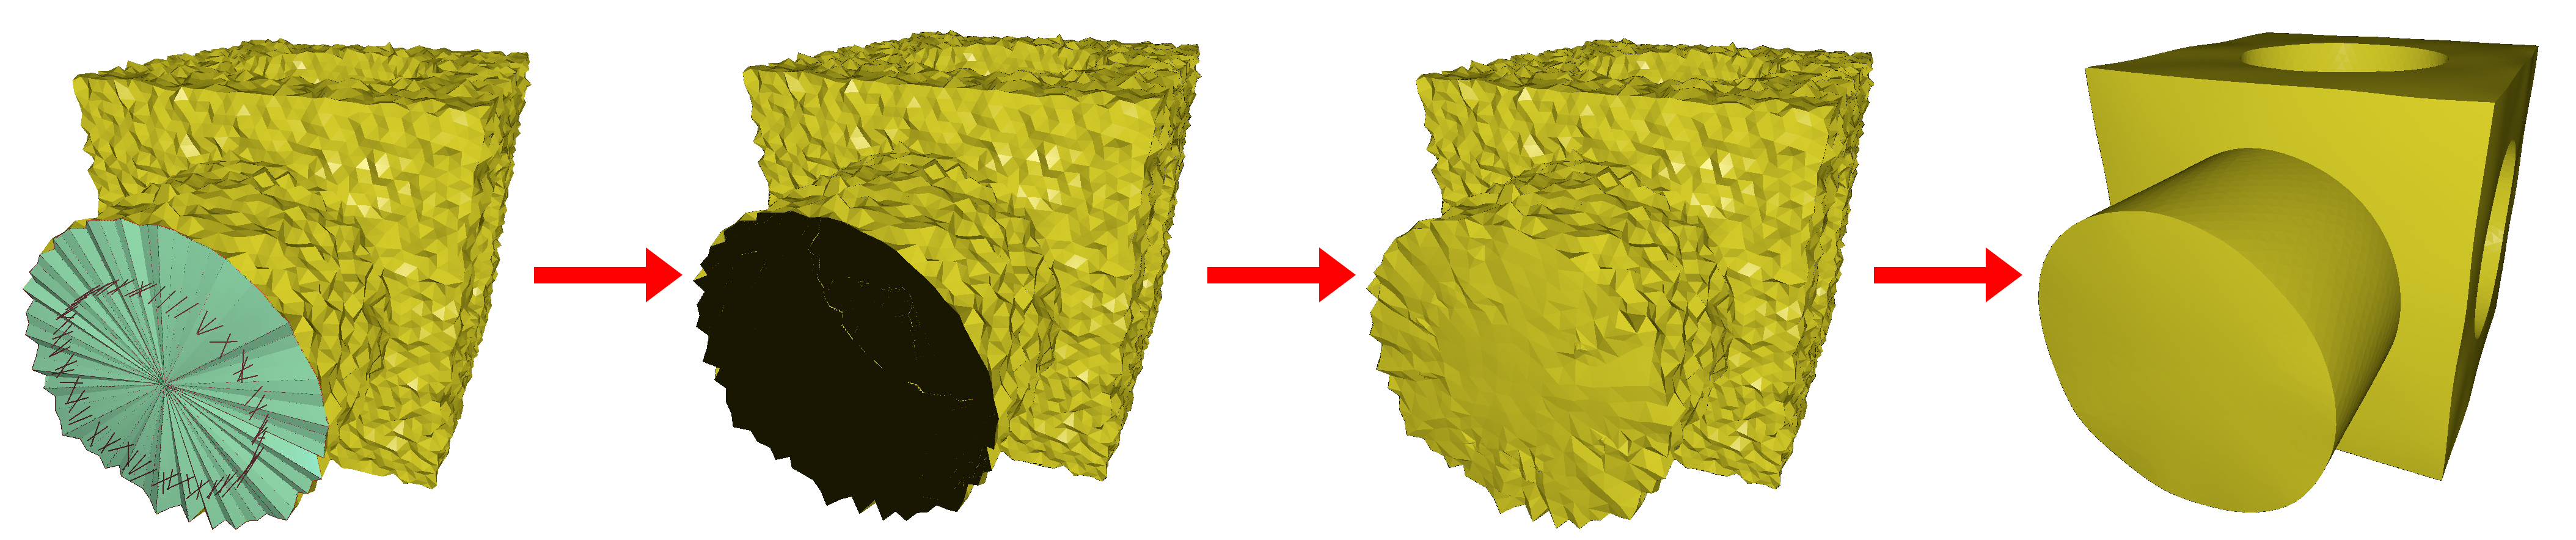
\includegraphics[width=\linewidth]{figuras/steps.png}
\caption{Fluxo geral da técnica proposta: Primeiramente é selecionado um ou mais \textit{patches} de faces de qualidade inferior às demais, representados pela cor verde clara na figura; em sequência esses \textit{patches} são apagados e melhores elementos são gerados em seu lugar. Como último passo, $k$ iterações são executadas intercalando o filtro bilateral nas normais das faces e a atualização da posição dos vértices baseado nessas normais filtradas.}
\label{fig:steps}
\end{figure}

\subsection{Pré-processamento}

Processos de aquisição de modelos 3D do mundo real algumas vezes não conseguem êxito na digitalização sem falhas do objeto, podendo ele ser processado com ruído e até mesmo ser gerado possuindo uma malha de elementos com qualidade insatisfatória. Como primeiro passo da técnica proposta, uma análise é feita na malha a ser processada. Este processo tem como objetivo identificar possíveis elementos que possam prejudicar o resultado final do filtro bilateral. A Figura \ref{fig:comparisonwithoutpreprocessing} exibe o resultado da aplicação da filtragem bilateral em um modelo que possui alguns elementos de qualidade ruim, mostrando assim a necessidade de um pré-processamento para que o modelo não aumente ou diminua seu volume e nem perca suas características provindas do modelo original.


\begin{figure}[!h]
\captionsetup{width=\linewidth}
\centering
\includegraphics[width=\linewidth]{figuras/comparison.png}
\caption{Filtro bilateral sem pré-processamento aplicado ao modelo \textit{block} com ruído artificial. Na área demarcada pode-se notar perda de característica do modelo original.}
\label{fig:comparisonwithoutpreprocessing}
\end{figure}


\subsubsection{Seleção de \textit{patches}}

Seja $M = (V,E,F)$ uma malha com ruído, onde $V$, $E$ e $F$ são os conjuntos de vértices, arestas e faces, respectivamente, de $M$. Um conjunto de faces (\textit{patches}) de $M$, que pode interferir no filtro bilateral, será então selecionado, de forma manual ou automática (Figura \ref{fig:validselection}) e extraído. Uma nova malha $M_p$ será então gerada contendo apenas os elementos deletados de $M$. No final deste processo (Figura \ref{fig:meshparts}) terão-se duas novas malhas: 

\begin{itemize}  
\item $M_p = (V_p,E_p,F_p)$, onde $V_p \subseteq V$, $E_p \subseteq E$ e $F_p \subseteq F$.
\item $M' = (V', E', F')$, resultante da extração dos \textit{patches} de $M$, onde $V' \subseteq V$, $E' \subseteq E$ e $F' = F - F_p$.
\end{itemize}


\begin{figure}[!h]
\captionsetup{width=\linewidth}
\centering
\includegraphics[scale=0.30]{figuras/validselection.png}
\caption{Uma seleção válida de \textit{patches} a serem utilizados no passo de pré-processamento. Em vermelho são mostradas as normais dos triângulos pertencentes aos \textit{patches} selecionados.}
\label{fig:validselection}
\end{figure}


Ainda no processo de deleção de \textit{patches}, a informação de fronteira de arestas é mantida para auxiliar na reconstrução dos elementos de $M'$. É então gerado um conjunto de arestas definido por:
\begin{equation} \label{eq:boundary} 
B = \{e : e \in (E_p \cap E')\}.
\end{equation}

\begin{figure}[!h]
\captionsetup{width=\linewidth}
\centering
\includegraphics[width=\linewidth]{figuras/meshparts.png}
\caption{Exemplo do processo de seleção de \textit{patches} e criação de novas malhas. Da esquerda para a direita: malha original com ruído $M$, malha suporte $M_p$ e malha $M'$.}
\label{fig:meshparts}
\end{figure}

\subsubsection{Reconstrução}

O segundo passo do pré-processamento é a reconstrução de $M'$. É descrito em \cite{miranda2009surface} uma técnica de reconstrução de malhas de superfície que considera curvaturas e seu algoritmo foi utilizado nesse passo do pré-processamento. Esta técnica é essencialmente um algoritmo de avanço de fronteira que gera elementos, em superfícies arbitrárias, com a melhor forma possível. 


\begin{figure}[!h]
\captionsetup{width=\linewidth}
\centering
\includegraphics[width=\linewidth]{figuras/meshregenerationoverview.jpg}
\caption{Visão geral do processo de geração de malha de superfície descrito em \cite{miranda2009surface}.}
\label{fig:meshregeneration}
\end{figure}

A Figura \ref{fig:meshregeneration} mostra a visão geral do método de geração de malha proposto. A entrada para o algoritmo é uma descrição poligonal do contorno da superfície a ser gerada a malha e uma superfície de suporte que é representada abstratamente por três métodos:

\begin{itemize}  
\item \textit{Primeiro método:} Dada uma posição de um ponto, o método retorna o tamanho característico desejado de um triângulo equilátero ideal a ser criado com nesta posição. O tamanho do lado do triângulo é considerado como tamanho característico.
\item \textit{Segundo método:} Dada uma aresta corrente na fronteira atual, o método localiza o ponto \textit{apex} ideal que forma um novo triângulo. O método tem dois argumentos de entrada: a altura do triângulo equilátero candidato e um vetor unitário perpendicular à direção da aresta base. 
\item \textit{Terceiro método:} Dado um ponto no espaço, o método retorna o ponto da superfície suporte mais próximo ao ponto dado. Este método é usado apenas no estágio final da geração de malha para melhoria da malha local.
\end{itemize}

A técnica se inicializa com um processo de avanço de fronteira na região de borda definida pelo conjunto $B$ (Equação \ref{eq:boundary}) e continua até que toda a região esteja com uma malha gerada. Para cada aresta base na fronteira ativa, será criado um novo triângulo, processo esse realizado da seguinte forma:

\begin{itemize}
    \item A posição ideal para o vértice de um triângulo equilátero a ser formado é determinado usando o \textit{Primeiro} e \textit{Segundo} métodos. Usando o ponto médio da aresta base corrente como entrada, o tamanho do lado de um triângulo equilátero, a ser formado naquela posição, é retornado pelo \textit{Primeiro} método. Com este tamanho, a altura do triângulo candidato é obtida. Então fazendo o produto vetorial entre a normal à superfície e a aresta da fronteira, definido apenas por: \textbf{Normal} $\times$ \textbf{Tangente}, é descoberto o vetor unitário perpendicular a ser utilizado no \textit{Segundo} método, que então retorna a posição ideal para o novo ponto a ser gerado. A Figura \ref{fig:meshgeneration} ilustra este processo.
\end{itemize}

\begin{figure}[!h]
\captionsetup{width=\linewidth}
\centering
\includegraphics[width=\linewidth]{figuras/meshgeneration.jpg}
\caption{Processo de encontrar a posição de um ponto ideal para a criação de um novo triângulo.}
\label{fig:meshgeneration}
\end{figure}


Como último passo, um processo de suavização é aplicado para aprimorar a qualidade da malha. Uma formulação para este passo é dado na Equação \ref{eq:meshlaplacian}, que é uma forma geral de um \textit{Laplaciano} com pesos atribuídos:

\begin{equation} \label{eq:meshlaplacian}
    X^{n+1}_O = X^{n}_O + \phi \frac{\sum^{m}_{i=1} w_{iO}(X^{n}_i - X^{n}_O) }{\sum^{m}_{i=1} w_{iO}},
\end{equation}
onde $m$ representa a quantidade de vértices conectados ao vértice $O$, $X^{n+1}_O$ é a posição do vértice $O$ na iteração $n+1$, $w_{iO}$ é o peso atribuído entre os vértices $i$ e $O$, e $\phi$ é um parâmetro de relaxamento normalmente determinado entre $(0,1]$. Em \cite{miranda2009surface} foi observado bons resultados com $\phi = w_{iO} = 1.0$, fazendo com que apenas os vértices adjacentes influenciem o vértice $O$. Esse processo de suavização geralmente faz com que os vértices se distanciem da superfície suporte. O \textit{Terceiro} método é utilizado com o intuito de reposicionar os vértices de volta à superfície suporte. Maiores detalhes podem ser encontrados em \cite{miranda2009surface}. 

Ao final deste processo de reconstrução, teremos como resultado uma malha $M_0$ com ruído, completamente pré-processada e pronta para ser utilizada no passo seguinte de remoção de ruídos do modelo.


\subsection{Processo de filtragem para otimização da malha}

Após o pré-processamento da malha, será utilizada uma técnica de remoção de ruídos no modelo que consistirá essencialmente em dois passos:

\begin{itemize}
    \item Aplicação da filtragem bilateral das normais das faces da malha;
    \item Reposicionamento dos vértices de acordo com as normais filtradas no passo anterior.
\end{itemize}


\subsubsection{Filtragem bilateral das normais das faces}

Manter as características do modelo é um grande desafio em uma técnica de filtragem bilateral. Filtrar diretamente os vértices da malha como descrito em \cite{fleishman2003bilateral} e \cite{jones2003non} pode ocasionar perdas de características importantes dependendo do modelo. Normais das faces de uma malha fornecem descrições mais precisas das características geométricas de um modelo. Uma aresta de borda pode ser detectada simplesmente calculando a diferença entre as normais das faces incidentes, como é ilustrado na Figura \ref{fig:meshsharpedge}. 

\begin{figure}[!h]
\captionsetup{width=\linewidth}
\centering
\includegraphics[width=\linewidth]{figuras/meshsharpedge.jpg}
\caption{Aresta AB de borda detectada pela grande diferença entre as normais das suas duas faces incidentes.}
\label{fig:meshsharpedge}
\end{figure}


Quando uma malha não possui ruído, as normais das faces podem fornecer um bom sinal guia na filtragem bilateral, no entanto, em um modelo com ruído, essa informação é perdida devido a grande divergência das normais presentes. O exemplo na Figura \ref{fig:meshpatchnormals} mostra que duas normais de triângulos vizinhos, compartilhando uma aresta, ainda podem ter valores muito divergentes de direção e essa aresta não ser de borda. É necessário então criar um conjunto de normais guia mais robusto que forneça informações geométricas mais precisas na presença de ruído.

\begin{figure}[!h]
\captionsetup{width=\linewidth}
\centering
\includegraphics[scale=0.83]{figuras/meshnormals.jpg}
\caption{Um \textit{patch} de triângulos de um modelo com ruído mostrando a divergência das normais de suas faces. Dessa forma, as normais não funcionam como um sinal guia confiável para a filtragem bilateral e não indicam informações geométricas precisas.}
\label{fig:meshpatchnormals}
\end{figure}

Um modelo baseado em malha pode ser decomposto em vários pequenos \textit{patches}, cada um consistindo de múltiplas faces com normais de direção similar. Decompor uma malha dessa forma não é intuitivo. Foi usado o mesmo processo descrito em \cite{zhang2015guided}: para cada face $f_k$ é definido um \textit{patch} $P_k$ como a união de $f_k$ e suas faces vizinhas que compartilham pelo menos um vértice com $f_k$. Para achar a normal guia de uma face $f_i$ é procurado dentre todos os \textit{patches} que $f_i$ faz parte, aquele que possui normais mais semelhantes, e então a normal média desse \textit{patch} é atribuída a $f_i$. O conjunto de \textit{patches} candidatos pode ser definido como:
\begin{equation}
    C(f_i) = \{P_k | f_i \in P_k\}.
\end{equation}
Para cada \textit{patch} $P \in C(f_i)$, é definida uma função de consistência que calcula o quão similares as normais no \textit{patch} $P$ são:
\begin{equation} \label{eq:consistencyfunc}
    H(P) = \Phi(P)\cdot R(P),
\end{equation}
onde $\Phi(P)$ mede a diferença máxima entre duas normais do \textit{patch}:
\begin{equation}
    \Phi(P) = \mathop{max}_{f_j,f_k \in P} \|\textbf{n}_j - \textbf{n}_k \| 
\end{equation}
e $R(P)$ é uma medida relativa de saliência de aresta no \textit{patch}:
\begin{equation}
    R(P) = \frac{max_{e_j\in E_p} \upvarphi(e_j)}{ \upvarepsilon + \sum_{e_j\in E_p}{\upvarphi(e_j)} },
\end{equation}
onde $E_p$ é o conjunto de arestas com ambas as faces incidentes contidas no \textit{patch} P (Figura \ref{fig:epedges}), $\upvarphi(e_j)$ mede a saliência de uma aresta $e_j$ pela diferença entre as normais das duas faces incidentes $f_{j_1}$ e $f_{j_2}$:
\begin{equation}
    \upvarphi(e_j) = \|\textbf{n}_{j_1} - \textbf{n}_{j_2} \|,
\end{equation}
e $\upvarepsilon$ é um valor positivo e pequeno para evitar divisões por $0$.

\begin{figure}[!h]
\captionsetup{width=\linewidth}
\centering
\includegraphics[scale=0.30]{figuras/E_pEdges.png}
\caption{Um \textit{patch} de faces e suas arestas. Linhas tracejadas ilustram as arestas pertencentes ao conjunto $E_p$.}
\label{fig:epedges}
\end{figure}

Entre todos os \textit{patches} candidatos para $f_i$, é escolhido o \textit{patch} $P^*$ que possui o menor valor para a função de consistência e é então computada a sua normal média $\mathbf{g}_i$, ponderada pela área das faces contidas no \textit{patch}:
\begin{equation}
    \mathbf{g}_i = \frac{ \sum_{f_j \in P^*}{A_j\mathbf{n}_j} }{ \|\sum_{f_j \in P^*}{A_j\mathbf{n}_j}\| },
\end{equation}
onde $A_j$ é a área da face $f_j$. Todo o processo é ilustrado na Figura \ref{fig:guidedzangconsistencyfunction}.

\begin{figure}[!h]
\captionsetup{width=\linewidth}
\centering
\includegraphics[width=\linewidth]{figuras/guidedzangconsistencyfunction.png}
\caption{Cálculo da função de consistência para todos os \textit{patches} que a face $f_i$ (em azul) está contida. O \textit{patch} $P$ com menor valor (destacado em vermelho) de função de consistência $H(P)$, calculado pela Equação \ref{eq:consistencyfunc}, será o escolhido, e sua normal média será atribuída à face $f_i$.}
\Fonte{\cite{zhang2015guided}}
\label{fig:guidedzangconsistencyfunction}
\end{figure}


Após a construção do conjunto de normais guia para toda a malha, o processo de filtragem irá prosseguir. Para cada face $f_i$, com vetor normal unitário $n_i$, centróide $c_i$, e normal guia $g_i$, é computado a normal filtrada $\overline{n}_i$ pelo seguinte filtro bilateral:
\begin{equation} \label{eq:filtrobilateraldasnormais}
    \overline{n}_i = \frac{1}{W_i}\sum_{f_j \in \mathcal{N}_i}{A_j K_s(c_i,c_j)K_r(g_i,g_j) n_j},
\end{equation}
onde $\mathcal{N}_i$ é o conjunto de faces na vizinhança de $f_i$; $A_j$ é a área da face $f_j$; \textbf{$K_s$} e \textbf{$K_r$} são os \textit{kernels} espacial e de distância respectivamente; \textbf{$n_j$} é a normal da face $f_j$ e $W_i = \|\sum_{f_j \in \mathcal{N}_i}{A_j K_s(c_i,c_j)K_r(g_i,g_j) n_j}\|$ é um fator de normalização para garantir que a normal filtrada será um vetor unitário. Para este trabalho, foram usadas as seguintes funções para \textbf{$K_s$} e \textbf{$K_r$}:
\begin{equation}
    K_s(c_i,c_j) = exp(-\frac{ {\| c_i-c_j \|}^2 }{ 2{\sigma_s}^2 }),
\end{equation}
\begin{equation}
    K_r(g_i,g_j) = exp(-\frac{ {\| g_i-g_j \|}^2 }{ 2{\sigma_r}^2 }),
\end{equation}
onde os parâmetros de variância \textbf{$\sigma_s$} e \textbf{$\sigma_r$} controlam a zona de influência dos \textit{kernels}. O conjunto $\mathcal{N}_i$ contém a face $f_i$ e suas faces vizinhas (Figura \ref{fig:facesvizinhas}). Elas podem ser definidas como:
\begin{itemize}
    \item \textbf{Vizinhas imediatas:} faces que compartilham pelo menos um vértice com $f_i$.
    \item \textbf{Vizinhas próximas:} faces cujo centróide está a uma distância $r$ do centróide de $f_i$.
\end{itemize}


\begin{figure}[!h]
\captionsetup{width=\linewidth}
\centering
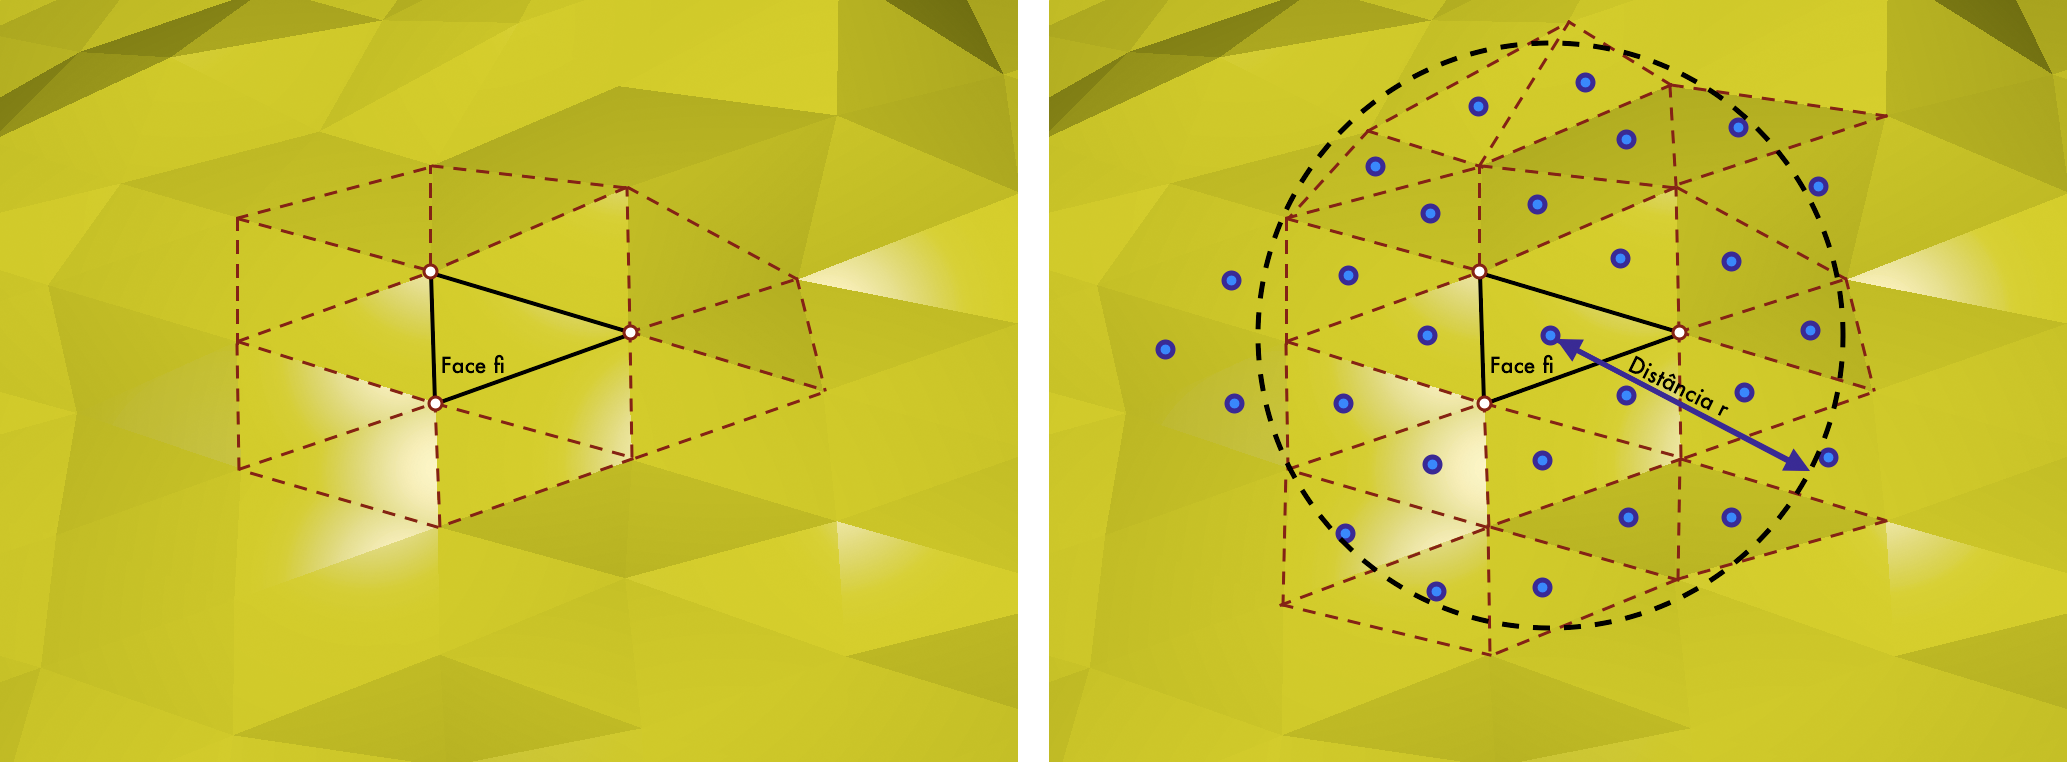
\includegraphics[width=\linewidth]{figuras/facesvizinhas.png}
\caption{Diferença da definição de vizinhança. A esquerda temos a vizinhança imediata de $f_i$; a direita, a vizinhança próxima de $f_i$, onde o parâmetro $r$, que representa o raio, é definido pelo usuário.}
\label{fig:facesvizinhas}
\end{figure}


\subsubsection{Atualizando vértices}

Após o processo de filtragem das normais, os vértices da malha têm que ser atualizados para corresponder às novas normais calculadas na Equação \ref{eq:filtrobilateraldasnormais}. Aqui foi usado o mesmo procedimento descrito em \cite{zhang2015guided} e \cite{sun2007fast}: para cada face $f_i$ com posições de vértice: $\overline{v}_{ix}$, $\overline{v}_{iy}$ e $\overline{v}_{iz}$, elas serão atualizadas pela seguinte iteração:
\begin{equation}
	\overline{v}^{(k+1)}_{i} = \overline{v}^{(k)}_{i} + \frac{1}{|\mathcal{F}_i|} \sum_{j \in \mathcal{F}_i}{ \overline{n}_j \Big[ \overline{n}_j \cdot \Big( \overline{c}^{(k)}_j - \overline{v}^{(k)}_i \Big) \Big] },
\end{equation}
onde $\overline{v}^{(k)}_{i}$ representa o valor de $\overline{v}_{i}$ na $k$-ésima iteração, $\mathcal{F}_i$ é o conjunto de índices das faces incidentes para o vértice $\overline{v}_{i}$ e $\overline{c}^{(t)}_j$ é o centróide de $f_i$ na $k$-ésima iteração. Esse procedimento é intercalado $k$ vezes com a filtragem das normais até que um resultado satisfatório seja obtido. Nos exemplos mostrados no capítulo seguinte, $k \in [10, 20]$ obteve bons resultados nos testes aplicados aos modelos.

O Algoritmo ~\ref{alg:finalmainalg} sumariza toda a técnica proposta no presente trabalho, mostrando os passos principais e omitindo detalhes que já foram discutidos ao longo do capítulo.

\begin{algorithm}[]
\SetKwInOut{Input}{Input}\SetKwInOut{Output}{Output}
\Input{Malha inicial $\mathbf{M}$, número de iterações $k$}
\Output{Malha $\mathbf{M_{k}}$ sem ruídos}
\BlankLine

    Selecione \textit{patches} \{p\} de faces em $\mathbf{M}$\;
    Delete o conjunto \{p\} de $\mathbf{M}$ gerando $\mathbf{M'}$ e $\mathbf{M_p}$\;
    Construa o conjunto $\mathbf{B}$ de fronteiras\;
    Gere $\mathbf{M_0}$ reconstruindo $\mathbf{M'}$ a partir de $\mathbf{B}$ e $\mathbf{M_p}$\;
    
    \Para{i = 1 até k}{
        Construa o conjunto de normais guia \{$\mathbf{g_i}$\}\;
        Compute as normais filtradas \{$\mathbf{\overline{n}_i}$\}\;
        Atualize os vértices de $\mathbf{M_i}$ de acordo com \{$\mathbf{\overline{n}_i}$\}\;
	}
    retorne $\mathbf{M_{k }}$\;
\caption{Filtragem Bilateral das normais da malha com passo de pré-processamento}
\label{alg:finalmainalg}
\end{algorithm}
